% To add an image or include a .tex file you need to add
% \CWD
% to the relative (to the main document) path.
%
% Example:

\begin{center}
\textit{
  A fauna de Minas Gerais é muito diversa. Além dos animais mais conhecidos, tamanduás-bandeira, tatus, lobos guará e onças pintada, em Minas Gerais também se pode encontrar centopéias. 
  }
\end{center}
  
  Ao andar pelo cerrado olhando atentamente para seus insetos, Elisa percebeu que a fauna de Minas é ainda mais diversa que o esperado, as "peias"  aqui não se limitam a centopeias ($100$-peias). Aqui temos $k$-peias: bichos com $k$ pés!
    
  Percebendo essa maravilha da natureza, Elisa decidiu fazer um desfile de $k$-peias para mostrar ao mundo o quão majestosas elas são. Para deixá-las ainda mais belas, Elisa decidiu que apenas participarão dos desfiles as $k$-peias que tiverem sapatos em \textbf{todos os seus $k$ pés}. 
  
  \begin{figure}[H]
    \centering
    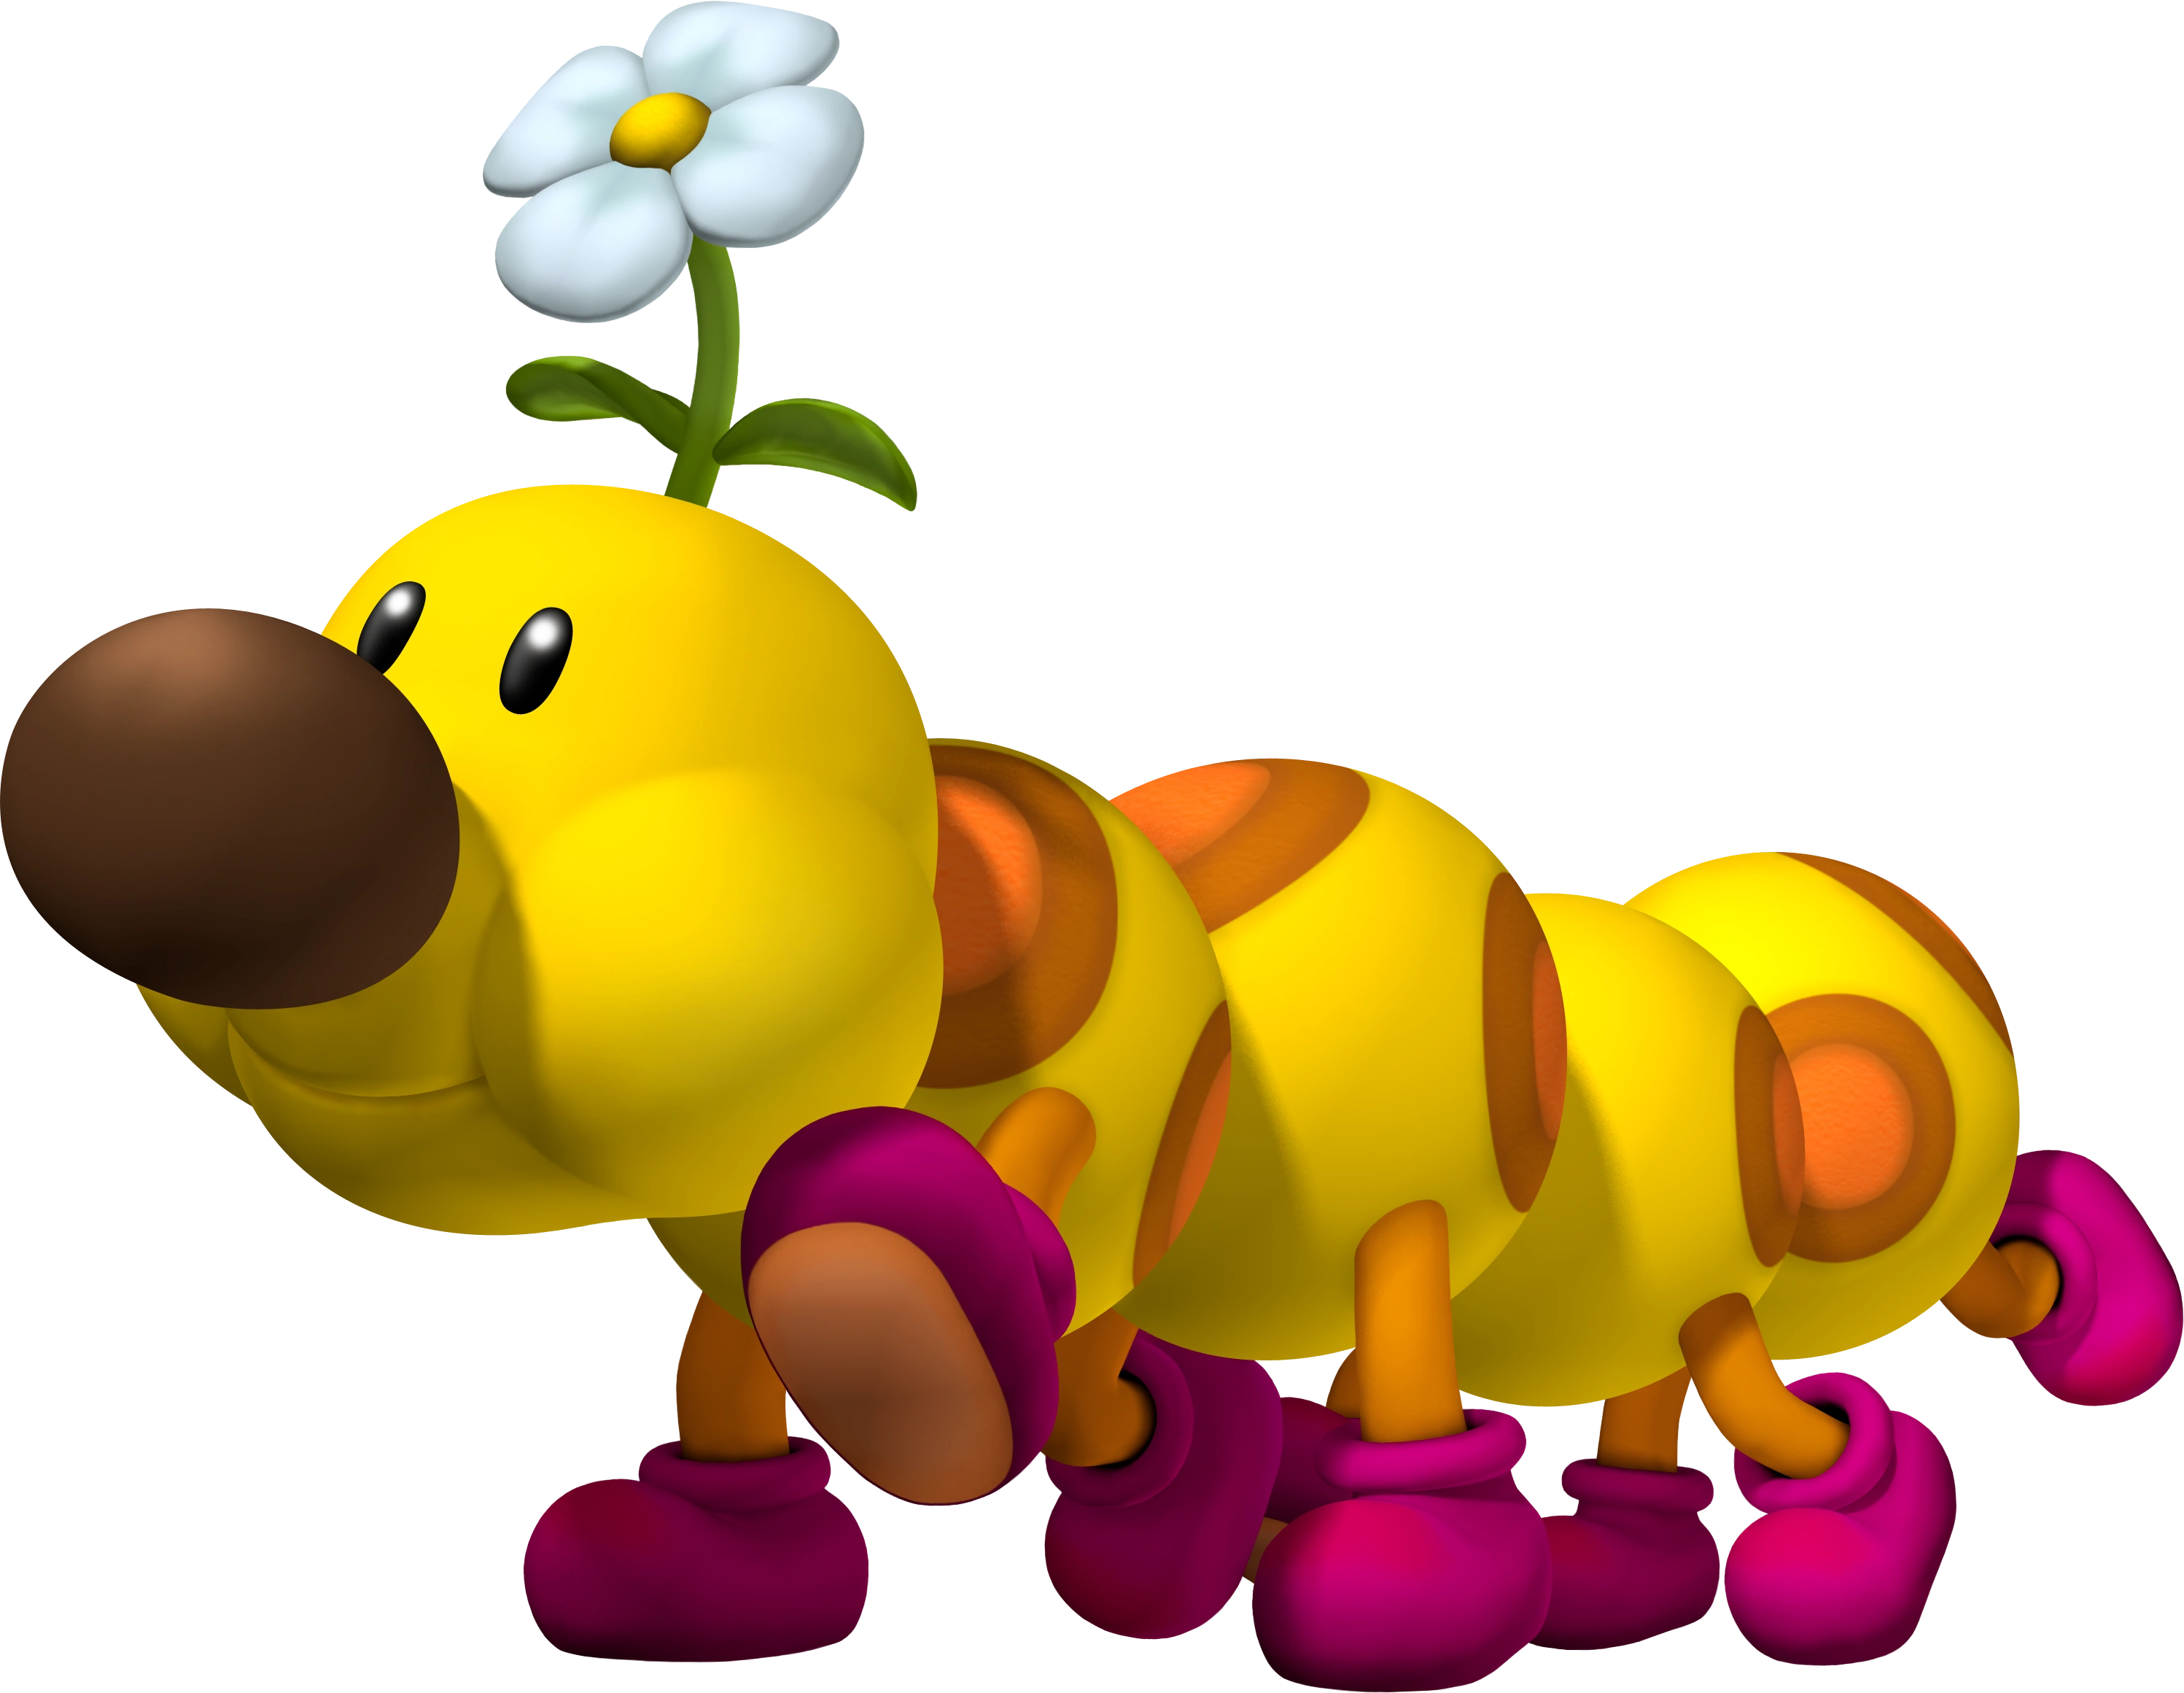
\includegraphics[width=5cm]{\CWD/8-peia.png}
    \caption{8-peia calçada.}
  \end{figure}

  Apesar de mais numerosos, os pés de $k$-peias são semelhantes aos pés humanos:
\begin{itemize}
  \item É garantido que o número $k$ de pés é par.
  \item Toda $k$-peia tem um tamanho de sapato $t$ que é o mesmo para todos os pés.
  \item Metade dos pés de uma $k$-peia são esquerdos e, a outra metade, direitos.
\end{itemize}

Dada que toda $k$-peia possui um número de "majestosidade"  (quão majestosa essa $k$-peia fica depois de calçada), ajude Elisa a distribuir seus sapatos de tal forma que a soma da majestosidade das $k$-peias seja maximizada.

% For input, use one of the following
%
\section*{Entrada}

A primeira linha possui dois números $1 \leq N \leq 500$ e $1 \leq T \leq 500$ o número de $k$-peias encontradas por Elisa e o tamanho máximo de seus sapatos, respectivamente.

Depois temos $N$ linhas descrevendo as $k$-peias. Na i-ésima delas temos três números $k_i$ ($2 \leq k_i \leq 100$), $t_i$ ($1 \leq t_i \leq T$) e $m_i$ ($1 \leq m_i \leq 10^9$): o número de pés da i-ésima $k$-peia, o tamanho dos seus pés e sua majestosidade, respectivamente. 

Por fim, teremos $T$ linhas sendo que a j-ésima delas contém números $e_j$ e $d_j$ ($0 \leq e_j, d_j \leq 50000$): quantos sapatos esquerdos e direitos de tamanho $j$ Elisa possui.

%
% For output, use one of the following
%


\section*{Saída}

Imprima uma única linha contendo a maior soma das majestosidades das $k$-peias se Elisa distribuir seus sapatos de forma ótima.

\section*{Restrições}

\begin{itemize}
\item $ 1 \leq N, T \leq 500$
\item $2 \leq k_i \leq 100$
\item $1 \leq t_i \leq T$
\item $1 \leq m_i \leq 10^9$
\end{itemize}

%\sampleio will look for files named sample-n.in and sample-n.sol (where n is 1, 2, 3...)
%in the documents directory and include them as samples.

\exemplo
